% !TeX root = ../../main.tex
\section{Smart Device}\label{section:smart-device}

The \enquote{Smart Device} is a part of the \ac{UBII} front end. It provides an interface for smart devices to provide data to different topics. The smart device is designed as a general purpose device. Only data of sensors which common smart devices have are provided. For more specific scenarios or devices, the smart device can not be used.

The \textbf{Web API} is used to fetch touch positions and events, orientation and acceleration from the device. This data is then sent to different topics using the \textbf{\ac{UBII} Client}. It is possible to set the view in full screen mode, to prevent unintentional interactions with control elements of the web browser or the operation system.

% describe orientational comes from the imu, 
%is interpolated, 
%but has limitations actually list limitations
%but is enough

% maybe show listing 

% note that it coul;d be derived from the gravitional vector and geometry.
The orientational data from the \textbf{Web API} 

% extend grafic um gamma and beta value, make smaller
\begin{figure}[htpb]
  \centering
  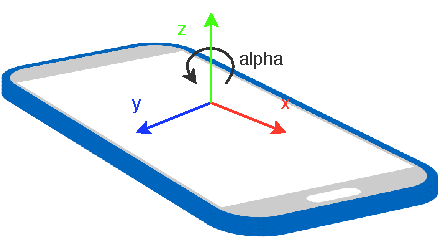
\includegraphics[width=12cm]{figures/device_orientation_alpha.pdf}
  \caption[Device Orientation]{The specification of the \lstinline{alpha} value visualized.}\label{fig:ubii_front_end}
\end{figure}


% why did i use it for this thesis?